%% %%%%%%%%%% %%%%%%%%%% %%%%%%%%%% %%%%%%%%%% %%%%%%%%%% %%%%%%%%%% %%%%%%%%%%

\section{Introduction}


    %% %%%%%%%%%% %%%%%%%%%% %%%%%%%%%% %%%%%%%%%% %%%%%%%%%% %%%%%%%%%% %%%%%%%%%%

    \begin{frame}[plain]{}

        \begin{center}

        \huge Introduction

        \end{center}

    \end{frame}


    %% %%%%%%%%%% %%%%%%%%%% %%%%%%%%%% %%%%%%%%%% %%%%%%%%%% %%%%%%%%%% %%%%%%%%%%

    \begin{frame}{Introduction}{Where are we? Where are we heading?}

%        \begin{itemize}
%
%            \item<1> Since its inception, there has been a sustained adoption of Information and Comunication Technologies% related devices and services, to support everyday human life
%
%            \item<2> Desktop and laptop computers, smartphones and tablets, wearable devices, datacenters to support on-line services
%
%            \item<3> ``Internet of Things'' is coming
%
%
%        \end{itemize}

        \begin{figure}[h]

            \centering

            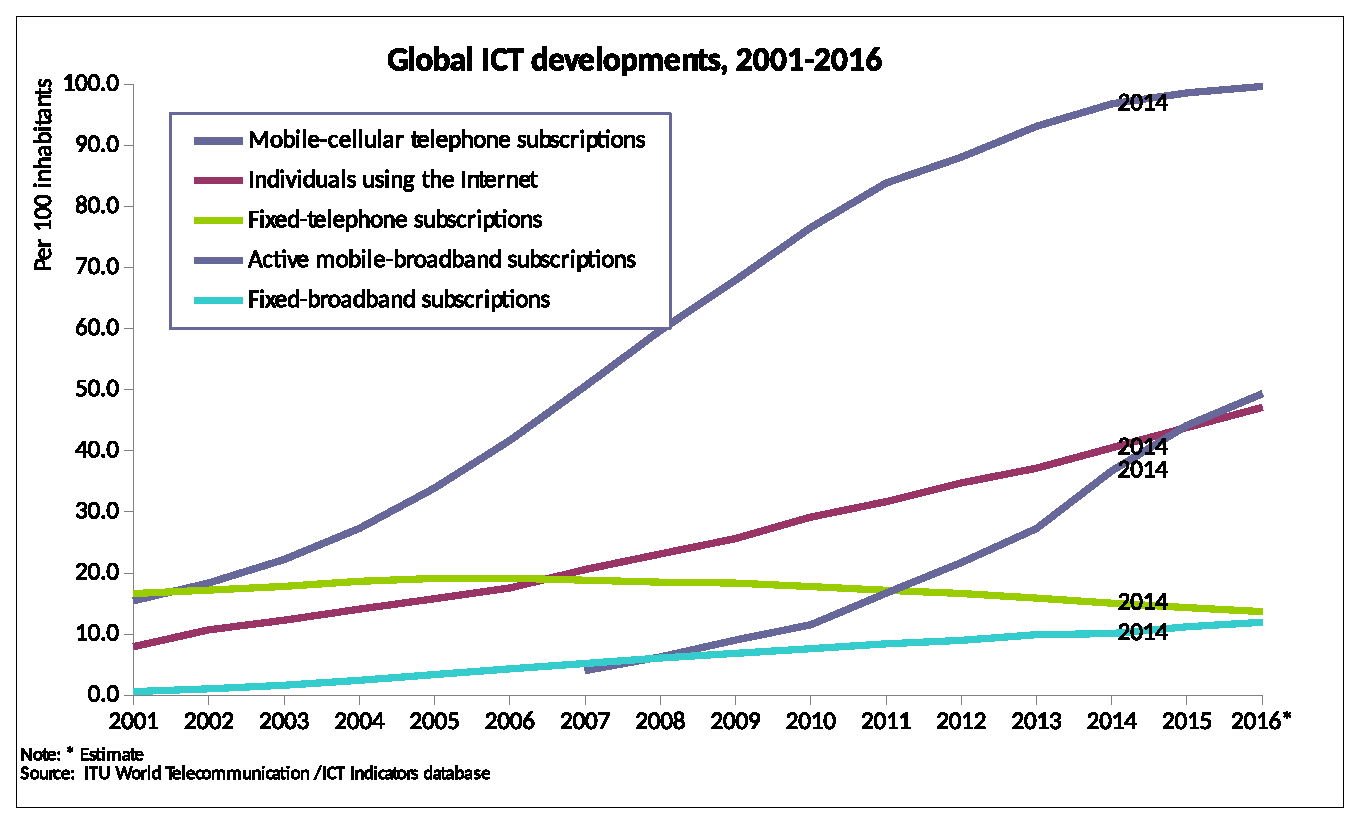
\includegraphics[width=1\textwidth]{images/ict_Developments-2001_2016} 

            \label{fig:ictAdoption}


        \end{figure}


    \end{frame}


    \begin{frame}{Introduction}{Where are we? Where are we heading?}

%        \begin{itemize}
%
%            \item<2> Desktop and laptop computers, smartphones and tablets, wearable devices, datacenters to support on-line services
%
%            \item<3> ``Internet of Things'' is coming
%
%
%        \end{itemize}

        \begin{figure}[h]

            \centering

$
            \begin{array}{ccc}

                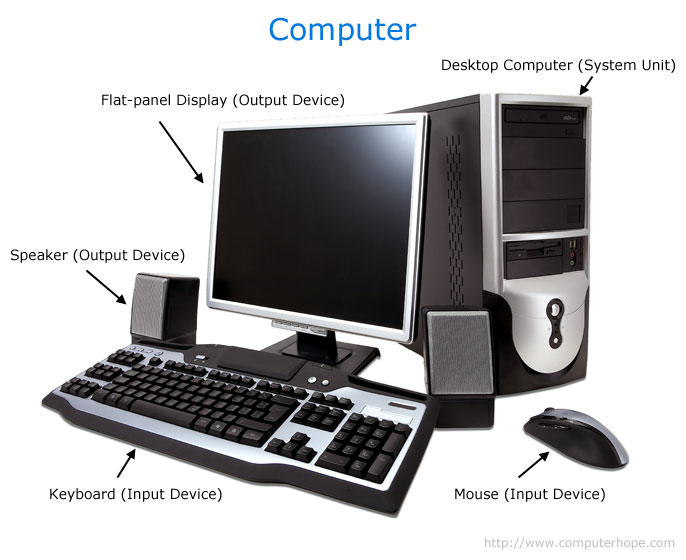
\includegraphics[scale=0.125]{images/desktop} &
                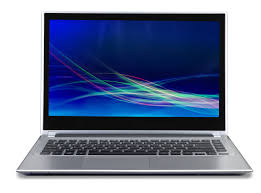
\includegraphics[scale=0.25]{images/laptop} &
                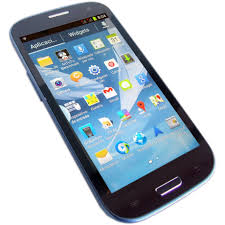
\includegraphics[scale=0.25]{images/smartphone}
                \\
                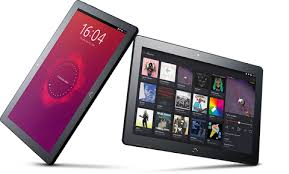
\includegraphics[scale=0.25]{images/tablet} &
                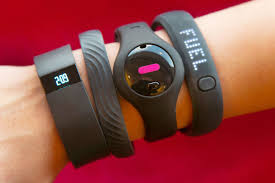
\includegraphics[scale=0.25]{images/wearable} &
                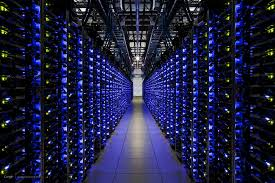
\includegraphics[scale=0.25]{images/data_center}


            \end{array}
$

            \label{fig:devices}


        \end{figure}


    \end{frame}


    \begin{frame}{Introduction}{Where are we? Where are we heading?}

%        \begin{itemize}
%
%            \item<3> ``Internet of Things'' is coming
%
%
%        \end{itemize}

        \begin{figure}[h]

            \centering

$
            \begin{array}{ccc}

            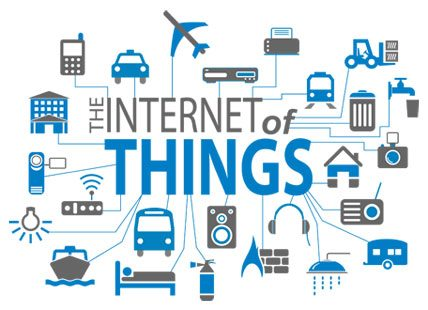
\includegraphics[scale=0.25]{images/internet-of-things}
            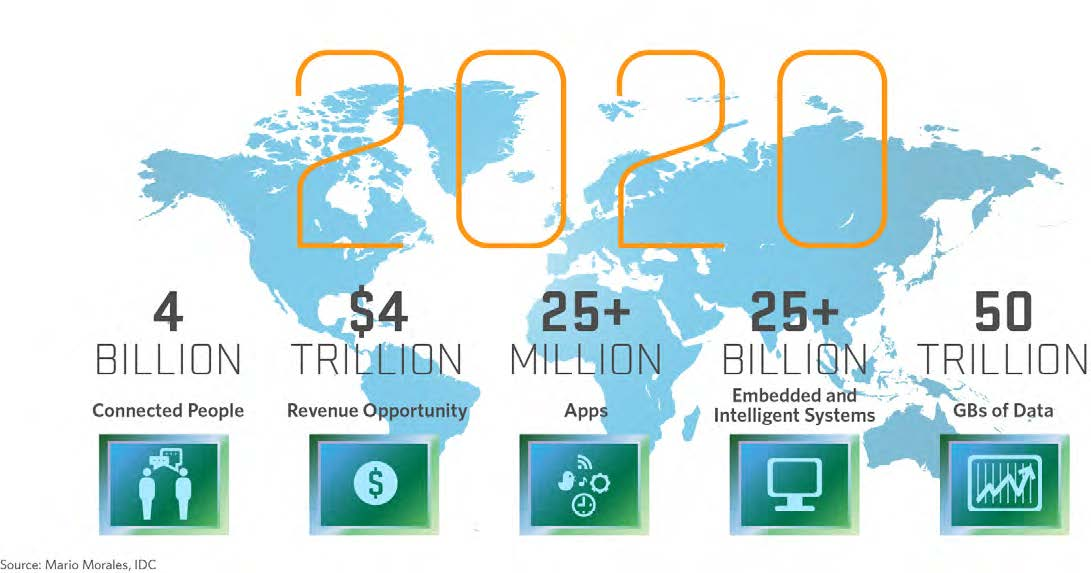
\includegraphics[scale=0.375]{images/internet-of-things-adoption-prediction}

            \end{array}
$

            \label{fig:internetOfThings}

        \end{figure}

        \vfill
        \footnotesize{Source: http://cdn2.business2community.com/wp-content/uploads/2016/06/internet-of-things.jpg}


    \end{frame}


    %% %%%%%%%%%% %%%%%%%%%% %%%%%%%%%% %%%%%%%%%% %%%%%%%%%% %%%%%%%%%% %%%%%%%%%%

    %\begin{frame}{Introduction}{And it's not going to stop!}


    %\end{frame}


    %% %%%%%%%%%% %%%%%%%%%% %%%%%%%%%% %%%%%%%%%% %%%%%%%%%% %%%%%%%%%% %%%%%%%%%%

    \begin{frame}{Introduction}{And the problem is\ldots}

        %This increase in device usage leads to the increase of:

%        \begin{itemize}
%
%            \item<1> Energy consumption
%
%            \item<2> Greenhouse gases emission
%
%            \item<3> Monetary costs% (derived from the previous items)
%
%        \end{itemize}

        \begin{figure}[h]

            \centering

            %\includegraphics[width=.75\textwidth]{images/world_energy_consumption} 
            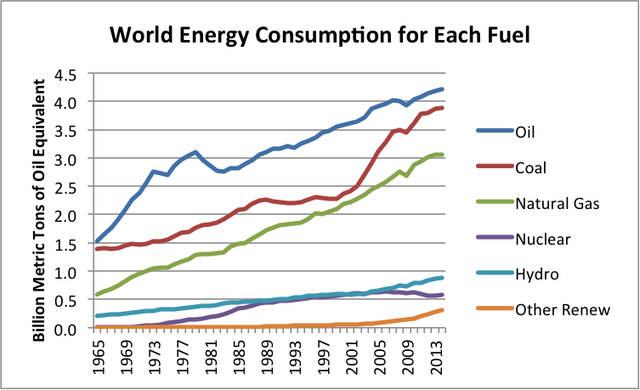
\includegraphics[width=.75\textwidth]{images/world-energy-consumption-for-each-fuel-2014-line} 

            \label{fig:worldEnergyConsumption}


        \end{figure}

        %\footnotesize{By Con-struct (BP Statistical Review of World Energy 2015) [GFDL (http://www.gnu.org/copyleft/fdl.html) or CC BY-SA 3.0 (http://creativecommons.org/licenses/by-sa/3.0)], via Wikimedia Commons}


        \footnotesize{Our Finite World blog by Gail Tverberg is licensed under a Creative Commons Attribution-ShareAlike 3.0 Unported License.}

    \end{frame}


    \begin{frame}{Introduction}{And the problem is\ldots}

        %This increase in device usage leads to the increase of:

%        \begin{itemize}
%
%            \item<2> Greenhouse gases emission
%
%            \item<3> Monetary costs% (derived from the previous items)
%
%        \end{itemize}

        \begin{figure}[h]

            \centering

$
            \begin{array}{cc}

            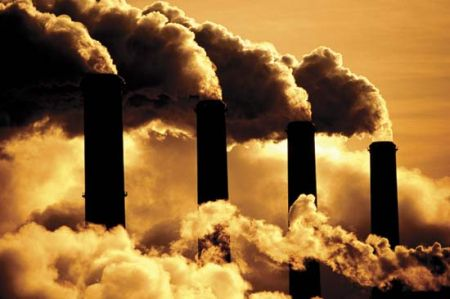
\includegraphics[width=.375\textwidth]{images/greenhouse-gas} &
            \includegraphics[width=.375\textwidth]{images/money-055}

            \end{array}
$

            \label{fig:greenhouseGasEmissionAndMoneyCosts}


        \end{figure}

        \footnotesize{DIBYANGSHU SARKAR/AFP/Getty Images}


    \end{frame}


%    \begin{frame}{Introduction}{And the problem is\ldots}
%
%        %This increase in device usage leads to the increase of:
%
%%        \begin{itemize}
%%
%%            \item<3> Monetary costs% (derived from the previous items)
%%
%%        \end{itemize}
%
%        \begin{figure}[h]
%
%            \centering
%
%            \includegraphics[width=.75\textwidth]{images/money-055} 
%
%            \label{fig:monetaryCosts}
%
%
%        \end{figure}
%
%
%    \end{frame}



    %% %%%%%%%%%% %%%%%%%%%% %%%%%%%%%% %%%%%%%%%% %%%%%%%%%% %%%%%%%%%% %%%%%%%%%%

    \begin{frame}{Introduction}{Some numbers\ldots}


        %The ICT sector alone, is responsible for:

%        \begin{itemize}
%
%            \item<1> 50\% of the energy costs of organizations
%
%            \item<2> 7\% of global energy consumption (expected to reach 14\% by 2020)
%
%
%        \end{itemize}

        %Enterprise energy costs

        \begin{figure}[h]

            \centering

$
            \begin{array}{cc}

            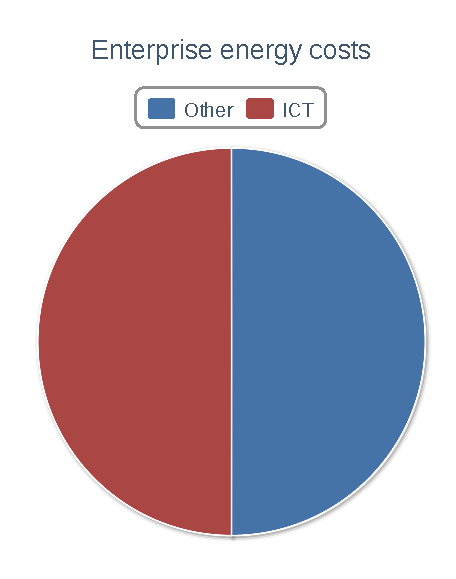
\includegraphics[width=.25\textwidth]{images/50-50} &
            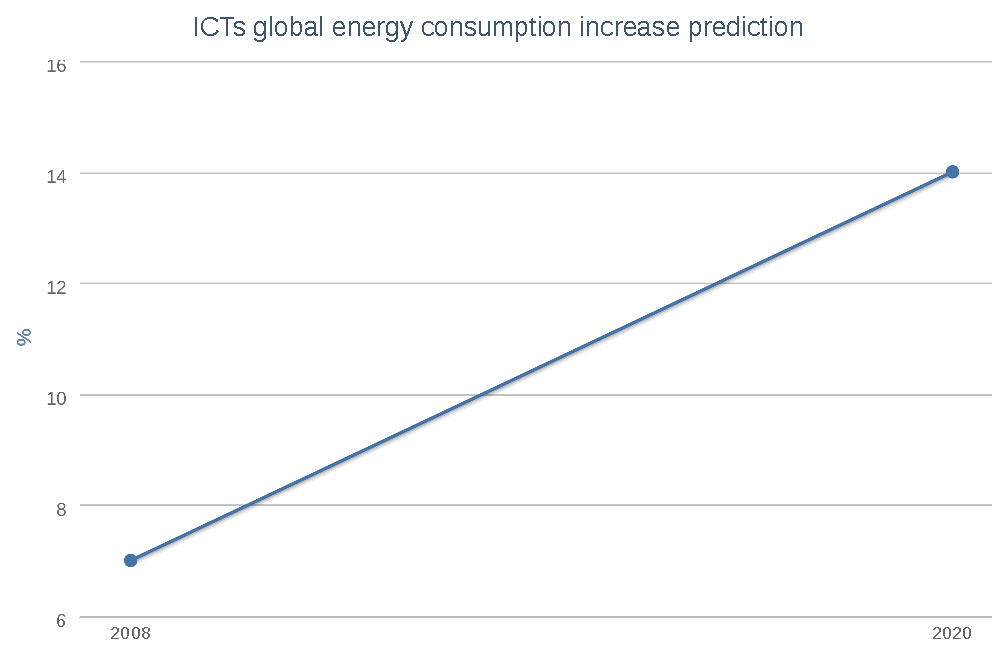
\includegraphics[width=.5\textwidth]{images/ictEnergyConsDoubleBy2020} 

            \end{array}
$

            \label{fig:entEnergyConsumption}


        \end{figure}


    \end{frame}


%    \begin{frame}{Introduction}{Some numbers\ldots}
%
%
%        %The ICT sector alone, is responsible for:
%
%%        \begin{itemize}
%%
%%            \item<2> 7\% of global energy consumption (expected to reach 14\% by 2020)
%%
%%
%%        \end{itemize}
%
%        ICTs global energy consumption increase prediction
%
%        \begin{figure}[h]
%
%            \centering
%
%            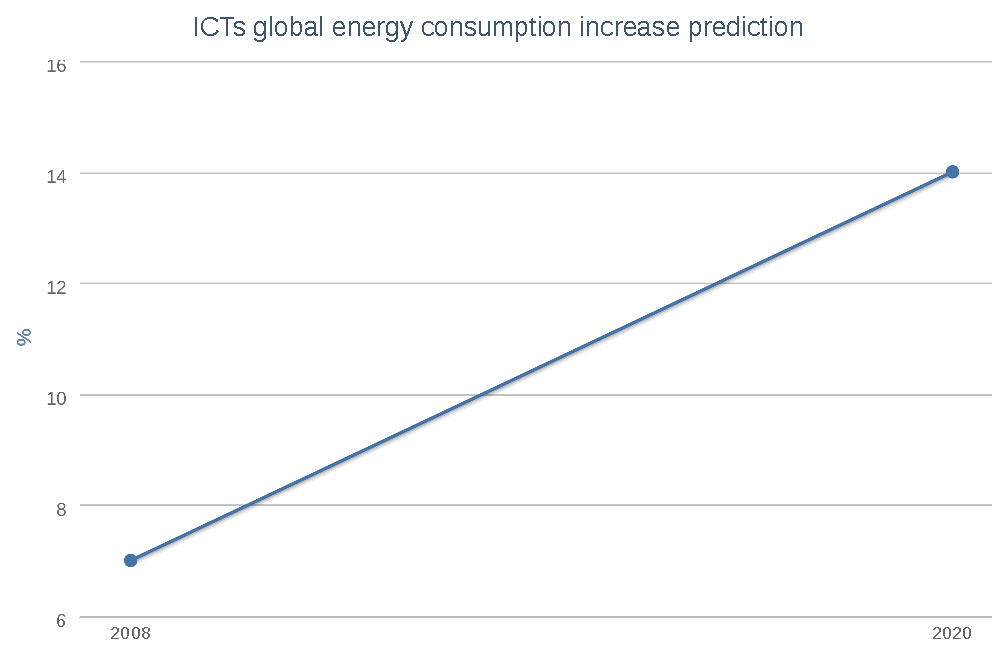
\includegraphics[width=.75\textwidth]{images/ictEnergyConsDoubleBy2020} 
%
%            \label{fig:ictEnergyConsDoubleBy2020}
%
%
%        \end{figure}
%
%
%    \end{frame}


    %% %%%%%%%%%% %%%%%%%%%% %%%%%%%%%% %%%%%%%%%% %%%%%%%%%% %%%%%%%%%% %%%%%%%%%%

    \begin{frame}{Introduction}{We must\ldots}

        %\begin{itemize}

            %\item ICTs help reduce energy/resource consumption in other, diverse, ``areas''


        %\end{itemize}
  
%        \begin{itemize}
%
%            \item Alleviate ICTs own energy footprint
%
%
%        \end{itemize}

        \begin{figure}[h]

            \centering

            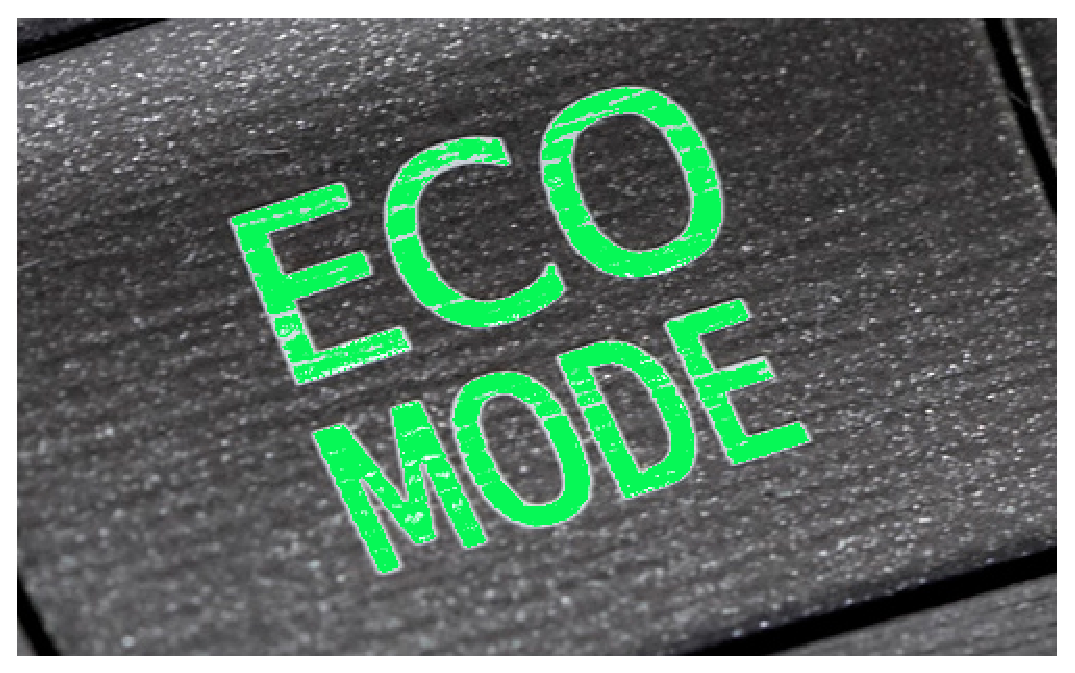
\includegraphics[width=.75\textwidth]{images/ecomode} 

            \label{fig:ecomode}


        \end{figure}


    \end{frame}


    %% %%%%%%%%%% %%%%%%%%%% %%%%%%%%%% %%%%%%%%%% %%%%%%%%%% %%%%%%%%%% %%%%%%%%%%

    \begin{frame}{Introduction}{We intend to\ldots}

        \begin{itemize}

            \item<1> Search possible gains in the energy consumption of software

            \item<2> Focus on the \Haskell language


        \end{itemize}

    \end{frame}


    %% %%%%%%%%%% %%%%%%%%%% %%%%%%%%%% %%%%%%%%%% %%%%%%%%%% %%%%%%%%%% %%%%%%%%%%

    \begin{frame}{Introduction}{We have\ldots}

        \begin{itemize}

            \item Investigated the \Edison library

            \begin{itemize}

                \item Refactoring, to use alternative data structure implementations

                \item Concerning Package and DRAM energy consumptions

		\item Compiler optimizations effect


            \end{itemize}

            \item http://green-haskell.github.io


        \end{itemize}


    \end{frame}


    %% %%%%%%%%%% %%%%%%%%%% %%%%%%%%%% %%%%%%%%%% %%%%%%%%%% %%%%%%%%%% %%%%%%%%%%

    \begin{frame}{Introduction}{Research Question!}


        \RQ{}. How do execution time and Package and RAM energy consumptions are affected by the use of a lazy or strict data structure implementation?
        %\medskip
        %\pause


    \end{frame}


    %% %%%%%%%%%% %%%%%%%%%% %%%%%%%%%% %%%%%%%%%% %%%%%%%%%% %%%%%%%%%% %%%%%%%%%%


%% %%%%%%%%%% %%%%%%%%%% %%%%%%%%%% %%%%%%%%%% %%%%%%%%%% %%%%%%%%%% %%%%%%%%%%


